\title{Product Specification \\
	\large Chess}
\date{\vspace{-5ex}}
\documentclass[letterpaper,11pt]{article}
\usepackage{graphicx}
\graphicspath{ {images/} }
\begin{document}
\maketitle
\section*{Product purpose}
The team has been tasked to program a chess application. The team will do it's best to create a fully functional chess application with all rules. The goal is to provide a chess aplication which will function as a traning ground, but also bring hours of joy and entertainment for chess enthusiast, newcomers and experts alike.
\section*{Functional requirements}
\begin{itemize}
	\item A player should be able to choose wether to play black or white
	\item The system should have a visible chess board with chess pieces which the player can move
	\item The system should calculate a player score based on performance during a chess game and display it
	\item System should validate player moves according to chess rules
	\item A player should be able to move chess pieces according to chess rules
	\item A player can select a chess piece by clicking it
	\item A player may choose another chess piece bly clicking on it
	\item A selected game piece must belong to the active player
	\item The player moves a piece by clicking and dragging it to desired tile
	\item A player should be able to forfeit a game at any point
	\item A game is ended immediately a player forfeits
	\item A confirmation window should pop up when a player forfeits
	\item The system should let the player play against another player locally
	\item A player should be able to play against a computer
	\item A player should be able to choose difficulty against computer
	\item A player should be able to undo moves on easy mode against computer
	\item The system should highlight possible moves for a chess piece when selected on easy mode against computer
	\item A player should be able to undo up to 3 moves against computer
	\item The gameboard will be reverted to the previous state when a move is undone
	\item A player should be able to knock out an enemy chess piece by doing a legal move onto a tile with an enemy chess piece
	\item The captured pieces should be displayed in a box next to the chess board
\end{itemize}

\section*{Non-functional requirements}
\begin{itemize}
	\item The application should be executable on most mainstream OS
\end{itemize}

\newpage
\section*{User stories}
\begin{itemize}
	\item As a user, I can choose wether to play as black or white.
	\item As a user, I can choose diffuculty against the computer.
	\item As a user, I can undo moves when playing on easy difficulty against the computer.
	\item As a user, I can view the highscores.
	\item As a user, I can close the application.
	\item As a user, I can view tips \& tricks
	\item As a user, I can move a pawn 2 squares the first time I move it, 1 square otherwise. I can't move it backwards or horizontally, and I can only knock out enemies diagonally. Special moves I can perform is "en passant".
	\item As a user, I can move a bishop horizontally and vertically as long it's not obstructed. I can't change direction the same turn. Special moves I can perform is "castling".
	\item As a user, I can move a knight either 2 squares horizontally and 2 square vertically, or 2 squares vertically and 1 square horizontally.
	\item As a user, I can move a bishop diagonally as long it's not obstructed. I can't change direction the same turn.
	\item As a user, I can move a king 1 square in every direction. I can't move the king into a position that checks him.
	\item As a user, I can move a queen in every direction as long she's not obstructed.
	\item As a user, I can forfeit a match.
\end{itemize}

\newpage
\section*{Use case diagram}
\begin{center}
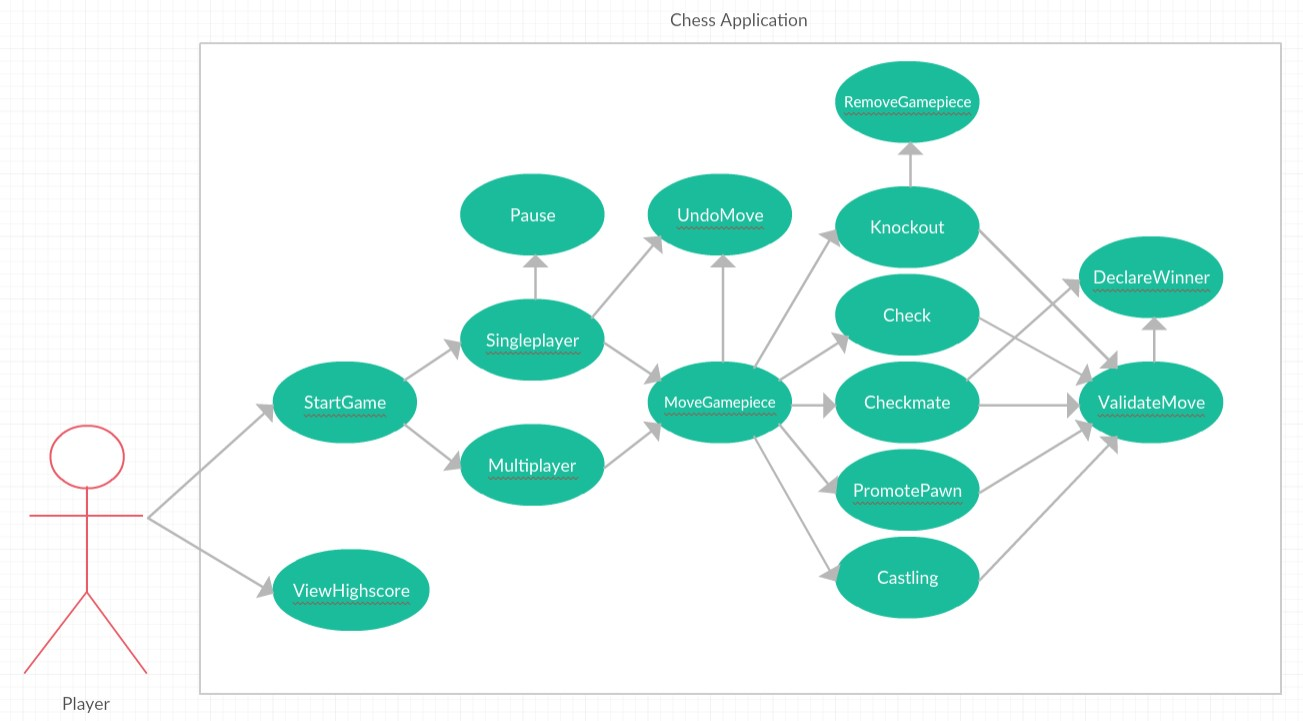
\includegraphics[width=16cm]{UseCaseDiagram}
\end{center}
\newpage
\section*{Fully dressed use case}

\begin{list}{}{}
	\item Use Case 1: Move chess piece
	\item Scope: Chess application
	\item Level: User goal
	\item Primary Actor: Player
	\item Stakeholders and Interests:
	\item \begin{list}{}{}
			\item Player: The player wants to be able to move his chess pieces accordingly to what the rules allows
			\item Programmer: The programmer wants the application to always follow the rules of a standard chess match
		\end{list}
	\item Preconditions: Player has started a game and it's the player's turn
	\item Postconditions: Player has successfully moved chosen chess piece and it's opponents turn
	\item Main Success Scenario:
	\item \begin{list}{}{}
			\item 1. It's player's turn. Player chooses piece to move.
			\item 2. Player drags chosen piece to desired square.
			\item 3. System validates player's move.
			\item 4. Player does a legal move and the chess piece stays on the chosen square
			\item 5. It's opponents turn
		\end{list}
	\item	Extensions:
	\item \begin{list}{}{}
			\item 4a: Illegal move
			\item \begin{list}{}{}
					\item 1. Player's chess piece is taken back if move is illegal
					\item 2. Player has to make a different move
				\end{list}
			\item 4b: Knocking out enemy piece
			\item \begin{list}{}{}
					\item 1. Player does a legal move and the chess piece lands on an enemy chess piece
					\item 2. Knocked out chess piece is removed from the board and displayed in the captured pieces window
					\item 3. Player's chess piece stays on the chosen square
				\end{list}
			\item 4c: Putting opponent into check
			\item \begin{list}{}{}
					\item 1. Player does a legal move and puts enemy king in check
					\item 2. Player's chess piece stays on the chosen square
					\item 3. Opponent MUST move their king out of check
				\end{list}
			\item 4d: Putting opponent into checkmate
			\item \begin{list}{}{}
					\item 1. Player does a legal move and puts enemy king in checkmate
					\item 2. Player wins the match
				\end{list}
		\end{list}
\end{list}


\begin{list}{}{}
	\item Use case 2: Player turn
	\item Scope: Chess application
	\item Level: User goal
	\item Primary Actor: Player
	\item Stakeholders and Interests:
	\item \begin{list}{}{}
			\item Player: The player wants to know what they can do when it's their turn
			\item Programmer: The programmer wants to ensure that the player is granted all possible options the player should have
		\end{list}
	\item Preconditions: Player has started a game and it's the player's turn
	\item Postconditions: Player's user input is executed
	\item Main Success Scenario:
	\item \begin{list}{}{}
			\item 1. It's the players turn
			\item 2. Player chooses piece and moves it
			\item 3. Opponents turn
		\end{list}
	\item Extensions:
	\item \begin{list}{}{}
			\item 2a: Pausing the game (against copmuter)
			\item \begin{list}{}{}
					\item 1. Player hits the pause button
					\item 2. Pause pop up appears
					\item 3. Application waits until player presses resume
				\end{list}
			\item 2b: Player forfeits (against computer)
			\item \begin{list}{}{}
					\item 1. Player hits the forfeit button
					\item 2. Confirmation pop up appears
					\item \begin{list}{}{}
							\item 2a. Player confirms forfeit
							\item \begin{list}{}{}
									\item 1. Match ends, player lose
									\item 2. Application goes back to main menu
								\end{list}
							\item 2b. Player cacncels forfeit
							\item \begin{list}{}{}
									\item 1. Match continues
								\end{list}
						\end{list}
				\end{list}
			\item 2c: Player forfeits (against another player)
			\item \begin{list}{}{}
					\item 1. Player hits the forfeit button
					\item 2. Confirmation pop up appears
					\item \begin{list}{}{}
							\item 2a. Other player accepts
							\item \begin{list}{}{}
									\item 1. Match ends, forfeiting player lose, other win
									\item 2. Application goes back to main menu
								\end{list}
							\item 2b. Other player cancels
							\item \begin{list}{}{}
									\item 1. Match continues
									\item 2. Forfeiting player can't forfeit until next turn
								\end{list}
						\end{list}
				\end{list}
			\item 2d: Draw by agreement
			\item \begin{list}{}{}
					\item 1. Player hits the draw button
					\item 2. Confirmation pop up appears
					\item \begin{list}{}{}
							\item 2a. Other player accepts
							\item \begin{list}{}{}
									\item 1. Match ends in draw, no winner
								\end{list}
							\item 2b. Other player declines
							\item \begin{list}{}{}
									\item 1. Match continues
									\item 2. Requesting player can't request another draw until next turn
								\end{list}
						\end{list}
				\end{list}
		\end{list}
\end{list}

\end{document}